% Options for packages loaded elsewhere
\PassOptionsToPackage{unicode}{hyperref}
\PassOptionsToPackage{hyphens}{url}
%
\documentclass[
]{book}
\usepackage{lmodern}
\usepackage{amssymb,amsmath}
\usepackage{ifxetex,ifluatex}
\ifnum 0\ifxetex 1\fi\ifluatex 1\fi=0 % if pdftex
  \usepackage[T1]{fontenc}
  \usepackage[utf8]{inputenc}
  \usepackage{textcomp} % provide euro and other symbols
\else % if luatex or xetex
  \usepackage{unicode-math}
  \defaultfontfeatures{Scale=MatchLowercase}
  \defaultfontfeatures[\rmfamily]{Ligatures=TeX,Scale=1}
\fi
% Use upquote if available, for straight quotes in verbatim environments
\IfFileExists{upquote.sty}{\usepackage{upquote}}{}
\IfFileExists{microtype.sty}{% use microtype if available
  \usepackage[]{microtype}
  \UseMicrotypeSet[protrusion]{basicmath} % disable protrusion for tt fonts
}{}
\makeatletter
\@ifundefined{KOMAClassName}{% if non-KOMA class
  \IfFileExists{parskip.sty}{%
    \usepackage{parskip}
  }{% else
    \setlength{\parindent}{0pt}
    \setlength{\parskip}{6pt plus 2pt minus 1pt}}
}{% if KOMA class
  \KOMAoptions{parskip=half}}
\makeatother
\usepackage{xcolor}
\IfFileExists{xurl.sty}{\usepackage{xurl}}{} % add URL line breaks if available
\IfFileExists{bookmark.sty}{\usepackage{bookmark}}{\usepackage{hyperref}}
\hypersetup{
  pdftitle={Knowledge Pool},
  pdfauthor={DAVeMoS team, Institut für Verkehrswesen (IVe), Universität für Bodenkultur Wien},
  hidelinks,
  pdfcreator={LaTeX via pandoc}}
\urlstyle{same} % disable monospaced font for URLs
\usepackage{longtable,booktabs}
% Correct order of tables after \paragraph or \subparagraph
\usepackage{etoolbox}
\makeatletter
\patchcmd\longtable{\par}{\if@noskipsec\mbox{}\fi\par}{}{}
\makeatother
% Allow footnotes in longtable head/foot
\IfFileExists{footnotehyper.sty}{\usepackage{footnotehyper}}{\usepackage{footnote}}
\makesavenoteenv{longtable}
\usepackage{graphicx,grffile}
\makeatletter
\def\maxwidth{\ifdim\Gin@nat@width>\linewidth\linewidth\else\Gin@nat@width\fi}
\def\maxheight{\ifdim\Gin@nat@height>\textheight\textheight\else\Gin@nat@height\fi}
\makeatother
% Scale images if necessary, so that they will not overflow the page
% margins by default, and it is still possible to overwrite the defaults
% using explicit options in \includegraphics[width, height, ...]{}
\setkeys{Gin}{width=\maxwidth,height=\maxheight,keepaspectratio}
% Set default figure placement to htbp
\makeatletter
\def\fps@figure{htbp}
\makeatother
\setlength{\emergencystretch}{3em} % prevent overfull lines
\providecommand{\tightlist}{%
  \setlength{\itemsep}{0pt}\setlength{\parskip}{0pt}}
\setcounter{secnumdepth}{5}
\usepackage{booktabs}
\usepackage{amsthm}
\makeatletter
\def\thm@space@setup{%
  \thm@preskip=8pt plus 2pt minus 4pt
  \thm@postskip=\thm@preskip
}
\makeatother
\usepackage[]{natbib}
\bibliographystyle{apalike}

\title{Knowledge Pool}
\author{DAVeMoS team, Institut für Verkehrswesen (IVe), Universität für Bodenkultur Wien}
\date{2021-11-16}

\begin{document}
\maketitle

{
\setcounter{tocdepth}{1}
\tableofcontents
}
\hypertarget{willkommen}{%
\chapter*{Willkommen}\label{willkommen}}
\addcontentsline{toc}{chapter}{Willkommen}


\includegraphics[width=0.4\linewidth]{image/davemos_logo}

Der Knowledge Pool ist eine sich ständig weiterentwickelnde Datenbank, die Teil des \href{https://www.davemos.online/}{DAVeMoS} Projekts ist. Sie zielt darauf ab, Konzepte und Belege für die systemischen Auswirkungen der Digitalisierung und Automatisierung des Verkehrs zu sammeln. Er ist ein Gemeinschaftswerk der DAVeMoS-Teammitglieder, die mit ihrem Fachwissen, ihren Ideen und Verbesserungsvorschlägen zu Inhalt und Design beigetragen haben:

\begin{itemize}
\tightlist
\item
  Dr.~Msc. MA (Hons) Martyna Bogacz
\item
  B.Sc. Veronika Hebenstreit
\item
  B.Sc. Gregor Husner
\item
  Univ. Prof.~Dr.~Yusak Susilo
\end{itemize}

Die Autoren freuen sich über Feedback, Fragen und Beiträge der Leser. Für weitere Eingaben wenden Sie sich bitte an die korrespondierende Autorin Martyna Bogacz unter der folgenden E-Mail-Adresse: \href{mailto:davemos.library@boku.ac.at}{\nolinkurl{davemos.library@boku.ac.at}}.


\includegraphics[width=0.1\linewidth]{image/cc}
This work is licensed under a Creative Commons Attribution-NonCommercial-NoDerivatives 4.0 International License.

The authors assume no responsibility or liability for any errors or omissions in the content of this work. The information contained in the knowledge pool is for general information purposes only.

\textbf{Inhaltsverzeichnis}

\begin{enumerate}
\def\labelenumi{\arabic{enumi}.}
\tightlist
\item
  \protect\hyperlink{intro}{Einleitung}
\item
  \protect\hyperlink{infrastructure}{Physische Straßeninfrastruktur}

  \begin{itemize}
  \tightlist
  \item
    \protect\hyperlink{dedicated_lanes}{Gesonderte Fahrspuren für vernetzte und automatisierte Fahrzeuge (connected and automated vehicles - CAV)}\\
  \item
    \protect\hyperlink{ODD}{Operative Gestaltungsbereiche}\\
  \item
    \protect\hyperlink{rail_crossing_info_system}{Informationssystem für Bahnübergänge}\\
  \item
    \protect\hyperlink{ers}{Elektrisches Straßensystem (Electric road system - ERS)}\\
  \item
    \protect\hyperlink{high_occupancy}{Fahrspuren für Fahrzeuge mit hoher Auslastung (high-occupancy vehicle - HOV)}\\
  \item
    \protect\hyperlink{public_trans_priority}{Prioritätssysteme für den öffentlichen Verkehr}\\
  \item
    \protect\hyperlink{transformation_public_space}{Transformation des öffentlichen Raums und digitale Lösungen}\\
  \end{itemize}
\item
  \protect\hyperlink{highway}{Verwaltung der Straßenverkehrsinfrastruktur}

  \begin{itemize}
  \tightlist
  \item
    \protect\hyperlink{uav}{Unbemannte Luftfahrzeuge für die Instandhaltung der Infrastruktur}\\
  \item
    \protect\hyperlink{charging_station}{Elektrische Ladestationen}\\
  \end{itemize}
\item
  \protect\hyperlink{traffic}{Traffic management}

  \begin{itemize}
  \tightlist
  \item
    \protect\hyperlink{congestion_charging}{Staugebühren (Congestion charging)}\\
  \item
    \protect\hyperlink{platooning}{Platooning}\\
  \item
    \protect\hyperlink{traffic_info_monitoring}{Verkehrsinformationen und -überwachung in Echtzeit}\\
  \item
    \protect\hyperlink{cits}{Kooperativ - intelligentes Verkehrssystem (Cooperative - intelligent transport system)}\\
  \item
    \protect\hyperlink{dynamic_route}{Dynamische Routenführung}\\
  \item
    \protect\hyperlink{variable_speed}{Variable Geschwindigkeitsbegrenzungen und dynamisches Beschilderungssystem}\\
  \item
    \protect\hyperlink{adaptive_traffic_control}{Intelligente Verkehrssignalsteuerung}\\
  \item
    \protect\hyperlink{p_g_fleet_management}{Flottenmanagement für Personentransport und Gütertransport}\\
  \item
    \protect\hyperlink{urban_access}{Verwaltung des städtischen Zugangs (Urban Access Management)}\\
  \end{itemize}
\item
  \protect\hyperlink{digital}{Digitale Straßeninfrastruktur und Konnektivität}

  \begin{itemize}
  \tightlist
  \item
    \protect\hyperlink{v2x}{V2X (Vehicle to everything / Fahrzeug-zu-Alles) Kommunikation}\\
  \item
    \protect\hyperlink{infrast_support_level}{Unterstützungsgrad der Infrastruktur für automatisiertes Fahren (ISAD - Infrastructure support for automated driving)}\\
  \end{itemize}
\item
  \protect\hyperlink{passenger}{Fahrgastinformationssystem}

  \begin{itemize}
  \tightlist
  \item
    \protect\hyperlink{djp}{Digitale Fahrplanauskunft}\\
  \item
    \protect\hyperlink{info_and_route_planning}{Multimodale Informationen und Routenplanung}\\
  \end{itemize}
\item
  \protect\hyperlink{multimodal}{Multimodales integriertes System}

  \begin{itemize}
  \tightlist
  \item
    \protect\hyperlink{flms}{Lösungen für die erste und letzte Meile}\\
  \item
    \protect\hyperlink{dist_time_fares}{Fahrpreise für den öffentlichen Personennahverkehr}\\
  \item
    \protect\hyperlink{maas}{Mobilität als Dienstleistung - Mobility as a service (Maas)}\\
  \item
    \protect\hyperlink{p_r}{Park and ride}\\
  \item
    \protect\hyperlink{contactless_cards}{Kontaktlose Karten für öffentliche Verkehrsmittel}\\
  \item
    \protect\hyperlink{special_needs}{Informationen und Unterstützung für Menschen mit besonderen Bedürfnissen}\\
  \item
    \protect\hyperlink{mobility_hubs}{Mobilitätszentren - Mobility hubs}\\
  \item
    \protect\hyperlink{rail_telematics}{Schienenverkehrstelematik für Passagiere und Güterverkehr}\\
  \end{itemize}
\item
  \protect\hyperlink{connected}{Automatisiertes Fahren}

  \begin{itemize}
  \tightlist
  \item
    \protect\hyperlink{av}{Automatisierte PKWs}
  \item
    \protect\hyperlink{parking_av}{Parkinfrastruktur für automatisierte Fahrzeuge}
  \item
    \protect\hyperlink{automated_road_freight}{Automatisierter Straßengüterverkehr}
  \item
    \protect\hyperlink{automatic_train}{Automatischer Zugbetrieb}\\
  \end{itemize}
\item
  \protect\hyperlink{onboard}{Bordtechnologie für vernetzte und automatisierte Fahrzeuge}

  \begin{itemize}
  \tightlist
  \item
    \protect\hyperlink{adas}{Fortschrittliche Fahrerassistenzsysteme (Advanced driver assistance system - ADAS)}\\
  \item
    \protect\hyperlink{parking_assistance}{Einparkhilfe-System}\\
  \item
    \protect\hyperlink{lane_keeping}{Spurhalte-Assistent}\\
  \item
    \protect\hyperlink{digital_maps}{Digitale Landkarten}\\
  \item
    \protect\hyperlink{ehorizon}{Electronic horizon}\\
  \item
    \protect\hyperlink{ecall}{Automatischer Notruf}\\
  \end{itemize}
\item
  \protect\hyperlink{freight}{Güterverkehr und gewerblicher Transport}

  \begin{itemize}
  \tightlist
  \item
    \protect\hyperlink{dangerous_goods}{Lokalisierung und Nachverfolgbarkeit von Waren}\\
  \item
    \protect\hyperlink{intermodal_freight}{Intermodaler Güterverkehr}\\
  \item
    \protect\hyperlink{urban_delivery}{Städtische Lieferungen}\\
  \item
    \protect\hyperlink{intelligent_truck_park}{Intelligentes LKW-Parken}\\
  \item
    \protect\hyperlink{space_book}{Intelligente Lieferflächenbuchung}\\
  \item
    \protect\hyperlink{delivery_drone}{Lieferdrohnen}\\
  \item
    \protect\hyperlink{electric_delivery_fleets}{Elektrofahrzeug-Lieferflotten}\\
  \item
    \protect\hyperlink{mtms}{Multimodale Verkehrsmanagementsysteme}\\
  \item
    \protect\hyperlink{freight_hubs}{Güterverkehrsknotenpunkte}\\
  \end{itemize}
\item
  \protect\hyperlink{collective}{Fahrzeuge der kollektiven Mobilität}

  \begin{itemize}
  \tightlist
  \item
    \protect\hyperlink{drt}{Bedarfsgesteuerte Verkehrssysteme (DRT -- Demand Responsive Transit)}\\
  \item
    \protect\hyperlink{prt}{Personenschnellverkehr (PRT - Personal Rapid Transit)}\\
  \item
    \protect\hyperlink{brt}{Busschnellverkehr (BRT - Bus rapid transit)}\\
  \item
    \protect\hyperlink{lrt}{Stadtbahnverkehr (LRT - Light Rail Transit)}\\
  \end{itemize}
\item
  \protect\hyperlink{big}{Big data}

  \begin{itemize}
  \tightlist
  \item
    \protect\hyperlink{wireless_com}{Drahtlose Kommunikationssysteme}\\
  \item
    \protect\hyperlink{bd_life}{Big data Lebenszyklus}
  \item
    \protect\hyperlink{bd_tool_maping}{Big-Data-Tools für die Kartierung und Vorhersage des Reiseverhaltens}\\
  \end{itemize}
\item
  \protect\hyperlink{shared}{Gemeinschaftliche Mobilität - Shared mobility}

  \begin{itemize}
  \tightlist
  \item
    \protect\hyperlink{car_sharing}{Car sharing}\\
  \item
    \protect\hyperlink{bike_sharing}{(E)-Fahrrad-Sharing}\\
  \item
    \protect\hyperlink{scooters}{E-Kick-Scooter}\\
  \item
    \protect\hyperlink{ride_hailing}{Fahrgemeinschaften (Ride-sharing)}\\
  \item
    \protect\hyperlink{passenger_drones}{Passagierdrohnen}
  \end{itemize}
\item
  \protect\hyperlink{alternative}{Alternative Energieträger}

  \begin{itemize}
  \tightlist
  \item
    \protect\hyperlink{FCEV}{Wasserstoff-Brennstoffzelle}\\
  \item
    \protect\hyperlink{bev}{Batterieelektrisch}\\
  \item
    \protect\hyperlink{plugin_hybrid}{Plugin-Hybridfahrzeuge}\\
  \end{itemize}
\item
  \protect\hyperlink{reference}{Referenzen}
\end{enumerate}

Der Knowledge Pool wurde zusammengestellt am:

\begin{verbatim}
## [1] "16 November 2021"
\end{verbatim}

\hypertarget{inhaltsverzeichnis}{%
\chapter*{Inhaltsverzeichnis}\label{inhaltsverzeichnis}}
\addcontentsline{toc}{chapter}{Inhaltsverzeichnis}

\begin{enumerate}
\def\labelenumi{\arabic{enumi}.}
\tightlist
\item
  \protect\hyperlink{intro}{Einleitung}
\item
  \protect\hyperlink{infrastructure}{Physische Straßeninfrastruktur}

  \begin{itemize}
  \tightlist
  \item
    \protect\hyperlink{dedicated_lanes}{Gesonderte Fahrspuren für vernetzte und automatisierte Fahrzeuge (connected and automated vehicles - CAV)}\\
  \item
    \protect\hyperlink{ODD}{Operative Gestaltungsbereiche}\\
  \item
    \protect\hyperlink{rail_crossing_info_system}{Informationssystem für Bahnübergänge}\\
  \item
    \protect\hyperlink{ers}{Elektrisches Straßensystem (Electric road system - ERS)}\\
  \item
    \protect\hyperlink{high_occupancy}{Fahrspuren für Fahrzeuge mit hoher Auslastung (high-occupancy vehicle - HOV)}\\
  \item
    \protect\hyperlink{public_trans_priority}{Prioritätssysteme für den öffentlichen Verkehr}\\
  \item
    \protect\hyperlink{transformation_public_space}{Transformation des öffentlichen Raums und digitale Lösungen}\\
  \end{itemize}
\item
  \protect\hyperlink{highway}{Verwaltung der Straßenverkehrsinfrastruktur}

  \begin{itemize}
  \tightlist
  \item
    \protect\hyperlink{uav}{Unbemannte Luftfahrzeuge für die Instandhaltung der Infrastruktur}\\
  \item
    \protect\hyperlink{charging_station}{Elektrische Ladestationen}\\
  \end{itemize}
\item
  \protect\hyperlink{traffic}{Traffic management}

  \begin{itemize}
  \tightlist
  \item
    \protect\hyperlink{congestion_charging}{Staugebühren (Congestion charging)}\\
  \item
    \protect\hyperlink{platooning}{Platooning}\\
  \item
    \protect\hyperlink{traffic_info_monitoring}{Verkehrsinformationen und -überwachung in Echtzeit}\\
  \item
    \protect\hyperlink{cits}{Kooperativ - intelligentes Verkehrssystem (Cooperative - intelligent transport system)}\\
  \item
    \protect\hyperlink{dynamic_route}{Dynamische Routenführung}\\
  \item
    \protect\hyperlink{variable_speed}{Variable Geschwindigkeitsbegrenzungen und dynamisches Beschilderungssystem}\\
  \item
    \protect\hyperlink{adaptive_traffic_control}{Intelligente Verkehrssignalsteuerung}\\
  \item
    \protect\hyperlink{p_g_fleet_management}{Flottenmanagement für Personentransport und Gütertransport}\\
  \item
    \protect\hyperlink{urban_access}{Verwaltung des städtischen Zugangs (Urban Access Management)}\\
  \end{itemize}
\item
  \protect\hyperlink{digital}{Digitale Straßeninfrastruktur und Konnektivität}

  \begin{itemize}
  \tightlist
  \item
    \protect\hyperlink{v2x}{V2X (Vehicle to everything / Fahrzeug-zu-Alles) Kommunikation}\\
  \item
    \protect\hyperlink{infrast_support_level}{Unterstützungsgrad der Infrastruktur für automatisiertes Fahren (ISAD - Infrastructure support for automated driving)}\\
  \end{itemize}
\item
  \protect\hyperlink{passenger}{Fahrgastinformationssystem}

  \begin{itemize}
  \tightlist
  \item
    \protect\hyperlink{djp}{Digitale Fahrplanauskunft}\\
  \item
    \protect\hyperlink{info_and_route_planning}{Multimodale Informationen und Routenplanung}\\
  \end{itemize}
\item
  \protect\hyperlink{multimodal}{Multimodales integriertes System}

  \begin{itemize}
  \tightlist
  \item
    \protect\hyperlink{flms}{Lösungen für die erste und letzte Meile}\\
  \item
    \protect\hyperlink{dist_time_fares}{Fahrpreise für den öffentlichen Personennahverkehr}\\
  \item
    \protect\hyperlink{maas}{Mobilität als Dienstleistung - Mobility as a service (Maas)}\\
  \item
    \protect\hyperlink{p_r}{Park and ride}\\
  \item
    \protect\hyperlink{contactless_cards}{Kontaktlose Karten für öffentliche Verkehrsmittel}\\
  \item
    \protect\hyperlink{special_needs}{Informationen und Unterstützung für Menschen mit besonderen Bedürfnissen}\\
  \item
    \protect\hyperlink{mobility_hubs}{Mobilitätszentren - Mobility hubs}\\
  \item
    \protect\hyperlink{rail_telematics}{Schienenverkehrstelematik für Passagiere und Güterverkehr}\\
  \end{itemize}
\item
  \protect\hyperlink{connected}{Automatisiertes Fahren}

  \begin{itemize}
  \tightlist
  \item
    \protect\hyperlink{av}{Automatisierte PKWs}
  \item
    \protect\hyperlink{parking_av}{Parkinfrastruktur für automatisierte Fahrzeuge}
  \item
    \protect\hyperlink{automated_road_freight}{Automatisierter Straßengüterverkehr}
  \item
    \protect\hyperlink{automatic_train}{Automatischer Zugbetrieb}\\
  \end{itemize}
\item
  \protect\hyperlink{onboard}{Bordtechnologie für vernetzte und automatisierte Fahrzeuge}

  \begin{itemize}
  \tightlist
  \item
    \protect\hyperlink{adas}{Fortschrittliche Fahrerassistenzsysteme (Advanced driver assistance system - ADAS)}\\
  \item
    \protect\hyperlink{parking_assistance}{Einparkhilfe-System}\\
  \item
    \protect\hyperlink{lane_keeping}{Spurhalte-Assistent}\\
  \item
    \protect\hyperlink{digital_maps}{Digitale Landkarten}\\
  \item
    \protect\hyperlink{ehorizon}{Electronic horizon}\\
  \item
    \protect\hyperlink{ecall}{Automatischer Notruf}\\
  \end{itemize}
\item
  \protect\hyperlink{freight}{Güterverkehr und gewerblicher Transport}

  \begin{itemize}
  \tightlist
  \item
    \protect\hyperlink{dangerous_goods}{Lokalisierung und Nachverfolgbarkeit von Waren}\\
  \item
    \protect\hyperlink{intermodal_freight}{Intermodaler Güterverkehr}\\
  \item
    \protect\hyperlink{urban_delivery}{Städtische Lieferungen}\\
  \item
    \protect\hyperlink{intelligent_truck_park}{Intelligentes LKW-Parken}\\
  \item
    \protect\hyperlink{space_book}{Intelligente Lieferflächenbuchung}\\
  \item
    \protect\hyperlink{delivery_drone}{Lieferdrohnen}\\
  \item
    \protect\hyperlink{electric_delivery_fleets}{Elektrofahrzeug-Lieferflotten}\\
  \item
    \protect\hyperlink{mtms}{Multimodale Verkehrsmanagementsysteme}\\
  \item
    \protect\hyperlink{freight_hubs}{Güterverkehrsknotenpunkte}\\
  \end{itemize}
\item
  \protect\hyperlink{collective}{Fahrzeuge der kollektiven Mobilität}

  \begin{itemize}
  \tightlist
  \item
    \protect\hyperlink{drt}{Bedarfsgesteuerte Verkehrssysteme (DRT -- Demand Responsive Transit)}\\
  \item
    \protect\hyperlink{prt}{Personenschnellverkehr (PRT - Personal Rapid Transit)}\\
  \item
    \protect\hyperlink{brt}{Busschnellverkehr (BRT - Bus rapid transit)}\\
  \item
    \protect\hyperlink{lrt}{Stadtbahnverkehr (LRT - Light Rail Transit)}\\
  \end{itemize}
\item
  \protect\hyperlink{big}{Big data}

  \begin{itemize}
  \tightlist
  \item
    \protect\hyperlink{wireless_com}{Drahtlose Kommunikationssysteme}\\
  \item
    \protect\hyperlink{bd_life}{Big data Lebenszyklus}
  \item
    \protect\hyperlink{bd_tool_maping}{Big-Data-Tools für die Kartierung und Vorhersage des Reiseverhaltens}\\
  \end{itemize}
\item
  \protect\hyperlink{shared}{Gemeinschaftliche Mobilität - Shared mobility}

  \begin{itemize}
  \tightlist
  \item
    \protect\hyperlink{car_sharing}{Car sharing}\\
  \item
    \protect\hyperlink{bike_sharing}{(E)-Fahrrad-Sharing}\\
  \item
    \protect\hyperlink{scooters}{E-Kick-Scooter}\\
  \item
    \protect\hyperlink{ride_hailing}{Fahrgemeinschaften (Ride-sharing)}\\
  \item
    \protect\hyperlink{passenger_drones}{Passagierdrohnen}
  \end{itemize}
\item
  \protect\hyperlink{alternative}{Alternative Energieträger}

  \begin{itemize}
  \tightlist
  \item
    \protect\hyperlink{FCEV}{Wasserstoff-Brennstoffzelle}\\
  \item
    \protect\hyperlink{bev}{Batterieelektrisch}\\
  \item
    \protect\hyperlink{plugin_hybrid}{Plugin-Hybridfahrzeuge}\\
  \end{itemize}
\item
  \protect\hyperlink{reference}{Referenzen}
\end{enumerate}

\hypertarget{intro}{%
\chapter{Einleitung}\label{intro}}

Diese Arbeit sammelt und definiert wesentliche Konzepte im Zusammenhang mit der Automatisierung und Digitalisierung des Verkehrssystems zusammen mit der Beschreibung ihrer Auswirkungen, sowohl negativ als auch positiv auf \textbf{individueller}, \textbf{systemischer} und \textbf{wirtschaftlicher Ebene}. Dieser Knowledge pool wird durch die Tatsache angetrieben, dass Automatisierung und Digitalisierung schnell voranschreiten, wenn auch nicht gleichmäßig in allen Bereichen im Verkehrskontext. Um das Spektrum der Möglichkeiten zu verstehen, die sie mit sich bringen, ist es daher notwendig, die Schlüsselkonzepte zu erklären, ihren Entwicklungsstand und ihre derzeitige Marktdurchdringung aufzuzeigen und schließlich ihre Auswirkungen auf verschiedenen Ebenen zu bewerten. Angesichts dieses Ansatzes enthält jedes Thema die folgenden \textbf{Definition} des Phänomens,
\textbf{Wichtige Interessensgruppen}, die für die jeweilige technologische Entwicklung verantwortlich und von ihr betroffen sind. Dann folgen zwei Unterabschnitte zum \textbf{aktuellen Stand der Forschung und Praxis}. Der erste Abschnitt fasst die neuesten Forschungsergebnisse zu einem bestimmten Thema zusammen, während der zweite Abschnitt den aktuellen Stand der Umsetzung einer bestimmten Technologie in der realen Welt erläutert. Der Abschnitt ``\textbf{Relevante Initiativen in Österreich}'' beschreibt die führenden Initiativen zu einem bestimmten Thema und das Potenzial für österreichische Akteure. Darüber hinaus bieten wir eine zusammenfassende Tabelle über die Auswirkungen des Konzepts auf ausgewählte \textbf{Ziele für nachhaltige Entwicklung} (SDGs). Um ein objektives Maß für den Entwicklungsstand der Technologie in den einzelnen Themenbereichen zu erhalten, haben wir außerdem die sogenannte \textbf{Technology Readiness Scale} (Williamson \& Beasley, 2011) wie unten beschrieben, integriert:

\begin{figure}
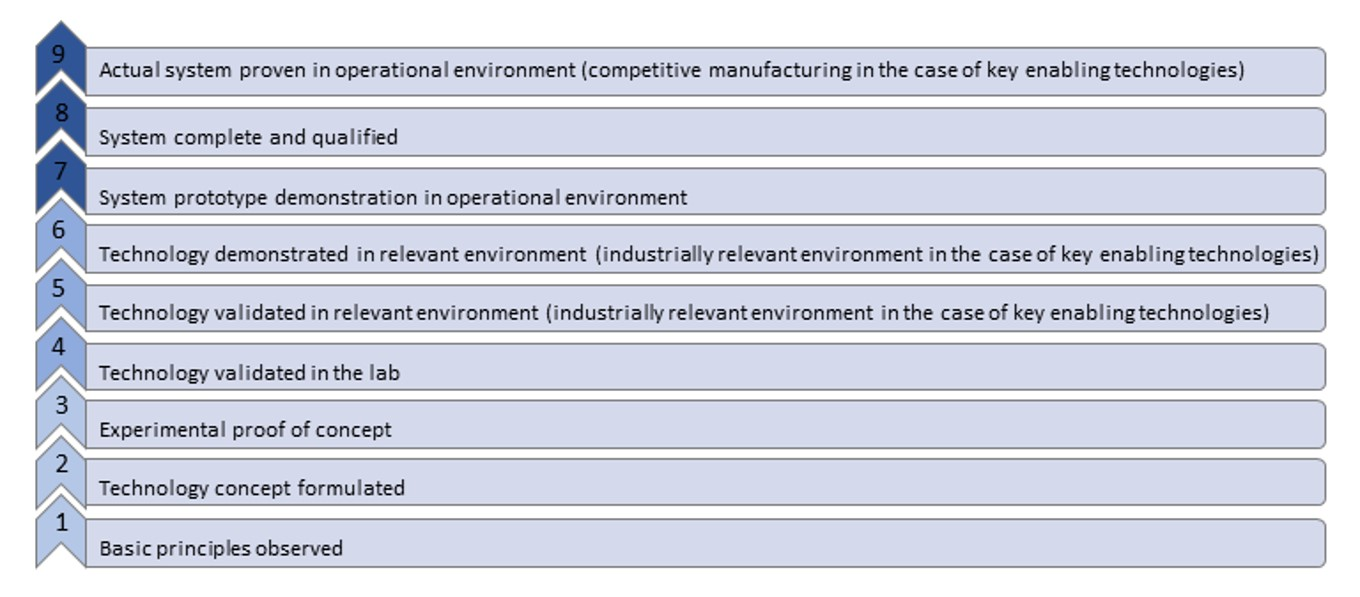
\includegraphics[width=0.8\linewidth]{image/TRL_cropped} \caption{Skala der technologischen Bereitschaft.}\label{fig:unnamed-chunk-4}
\end{figure}

Darüber hinaus bewerten wir die Bereitschaft einer bestimmten Technologie, in der Gesellschaft akzeptiert zu werden, und wie gut sie zum Gemeinwohl beiträgt, indem wir die \textbf{Skala der gesellschaftlichen Bereitschaft} verwenden (McCulloch, 2019):

\begin{figure}
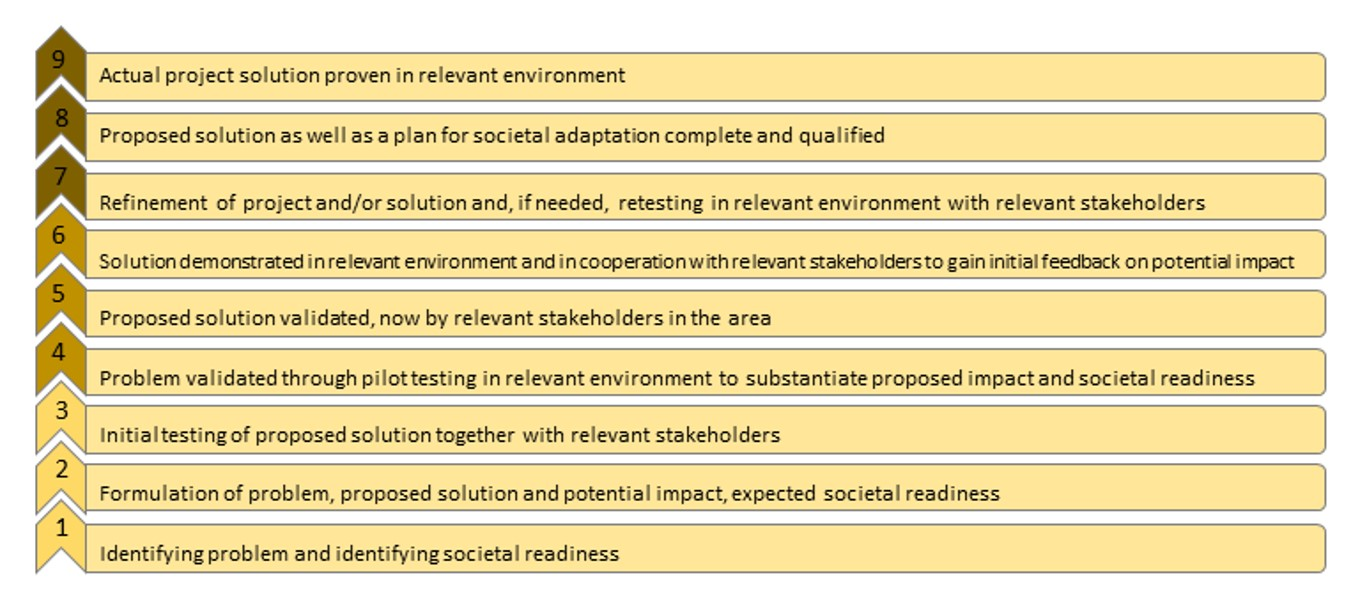
\includegraphics[width=0.8\linewidth]{image/SRL_cropped} \caption{Skala fuer die gesellschaftliche Bereitschaft.}\label{fig:unnamed-chunk-5}
\end{figure}

Abschließend finden Sie eine Liste \textbf{offener Fragen} und \textbf{Links zu weiteren Quellen} zu diesem Thema.

\textbf{Referenzen}

\begin{itemize}
\tightlist
\item
  Williamson, R., \& Beasley, J. (2011). \emph{Automotive technology and manufacturing readiness levels: a guide to recognised stages of development within the automotive industry}. URN11/672.
\item
  McCulloch, S. (2019). Social Acceptance And Societal Readiness Levels. \emph{DecarboN8}. Available at: \url{https://decarbon8.org.uk/social-acceptance-and-societal-readiness-levels/\#:~:text=Societal\%20readiness\%20refers\%20to\%20the,contributes\%20to\%20the\%20public\%20good.} {[}Accessed: 21 January 2021{]}.
\end{itemize}

  \bibliography{book.bib,packages.bib}

\end{document}
